\tikzset{every picture/.style={line width=0.75pt}} %set default line width to 0.75pt        

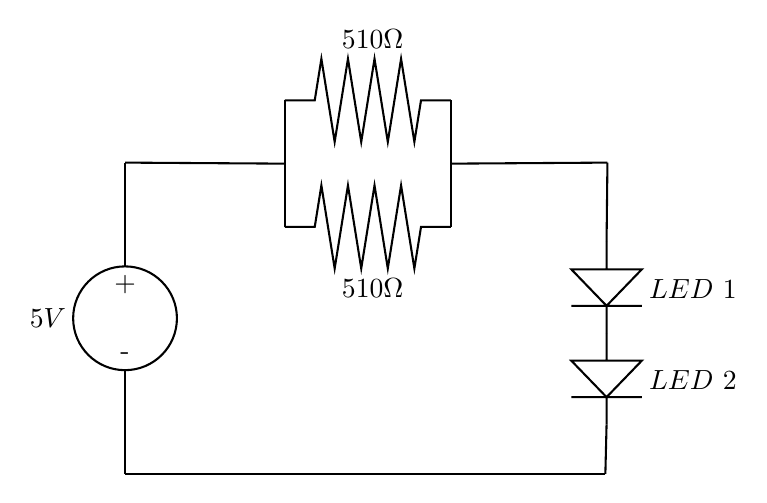
\begin{tikzpicture}[x=0.75pt,y=0.75pt,yscale=-1,xscale=1]
%uncomment if require: \path (0,536); %set diagram left start at 0, and has height of 536

%Shape: Circle [id:dp5391891321479709] 
\draw   (100,150) .. controls (100,136.19) and (111.19,125) .. (125,125) .. controls (138.81,125) and (150,136.19) .. (150,150) .. controls (150,163.81) and (138.81,175) .. (125,175) .. controls (111.19,175) and (100,163.81) .. (100,150) -- cycle ;
%Straight Lines [id:da29466546451147524] 
\draw    (125,175) -- (125,225) ;
%Straight Lines [id:da8075537755444633] 
\draw    (125,75) -- (125,125) ;
%Straight Lines [id:da5849282817970671] 
\draw    (357.42,75) -- (357,113.2) ;
%Straight Lines [id:da12428704129603618] 
\draw    (357,201.2) -- (356.42,225) ;
%Shape: Resistor [id:dp8585859917231262] 
\draw   (202,45) -- (216.4,45) -- (219.6,25) -- (226,65) -- (232.4,25) -- (238.8,65) -- (245.2,25) -- (251.6,65) -- (258,25) -- (264.4,65) -- (267.6,45) -- (282,45) ;
%Shape: Resistor [id:dp15449677573718512] 
\draw   (202,106) -- (216.4,106) -- (219.6,86) -- (226,126) -- (232.4,86) -- (238.8,126) -- (245.2,86) -- (251.6,126) -- (258,86) -- (264.4,126) -- (267.6,106) -- (282,106) ;
%Straight Lines [id:da07488249960137638] 
\draw    (202,45) -- (202,106) ;
%Straight Lines [id:da5526259810987513] 
\draw    (282,45) -- (282,106) ;
%Straight Lines [id:da2112986632937388] 
\draw    (125,75) -- (202,75.5) ;
%Straight Lines [id:da0027222316083801434] 
\draw    (282,75.5) -- (357.42,75) ;
%Shape: Diode [id:dp28676301231572787] 
\draw   (374,126.4) -- (357,144) -- (340,126.4) -- (374,126.4) -- cycle (357,113.2) -- (357,126.4) (374,144) -- (340,144) (357,144) -- (357,157.2) ;
%Shape: Diode [id:dp4391606122805669] 
\draw   (374,170.4) -- (357,188) -- (340,170.4) -- (374,170.4) -- cycle (357,157.2) -- (357,170.4) (374,188) -- (340,188) (357,188) -- (357,201.2) ;

%Straight Lines [id:da5657229854791843] 
\draw    (356.42,225) -- (125,225) ;

% Text Node
\draw (98,150) node [anchor=east] [inner sep=0.75pt]   [align=left] {5$\displaystyle V$};
% Text Node
\draw (125,128) node [anchor=north] [inner sep=0.75pt]   [align=left] {\begin{minipage}[lt]{8.68pt}\setlength\topsep{0pt}
\begin{center}
+
\end{center}

\end{minipage}};
% Text Node
\draw (125,172) node [anchor=south] [inner sep=0.75pt]   [align=left] {\begin{minipage}[lt]{8.67pt}\setlength\topsep{0pt}
\begin{center}
\mbox{-}
\end{center}

\end{minipage}};
% Text Node
\draw (228,129.4) node [anchor=north west][inner sep=0.75pt]    {$510\Omega $};
% Text Node
\draw (228,21.6) node [anchor=south west] [inner sep=0.75pt]    {$510\Omega $};
% Text Node
\draw (376,129.8) node [anchor=north west][inner sep=0.75pt]    {$LED\ 1$};
% Text Node
\draw (376,173.8) node [anchor=north west][inner sep=0.75pt]    {$LED\ 2$};


\end{tikzpicture}
